\chapter{Fundamentação Teórica}
\label{cap2}

O conceito de computação em nuvem (Seção~\ref{cap2:nuvem}) embora tenha vários aspectos amplamente conhecidos, normalmente possui as suas especificações desconhecidas para o grande público. 
%
Neste sentido, torna-se necessário entender os modelos de serviços, modelos de implantação e uma arquitetura de referência.
%
A implantação de uma nuvem emprega tecnologias de virtualização, que apesar de não serem uma tecnologia recente, é parte comum à softwares gerenciadores de nuvem, e portanto, a compreensão do comportamento de uma nuvem computacional está diretamente ligado à entender sobre o processo de virtualização.

Uma das aplicações da computação em nuvem é a consolidação de servidores, que consiste na instalação de um software responsável por gerenciar nuvens computacionais, que no caso de nuvens \ac{iaas} um dos softwares mais populares é o OpenStack (Seção \ref{cap2:openstack}).
%
O processo de consolidação deve levar em conta a arquitetura necessária para a instalação do OpenStack, ou seja, aprender sobre as funcionalidades oferecidas pelo software, como elas se comportam, e também como organizar a infraestrutura física é importante para garantir seu funcionamento.
%
Para entender o comportamento de uma nuvem computacional, uma análise minuciosa dos seus componentes torna-se necessária.
%
Sendo assim, para entender, por exemplo, o comportamento em uma das redes na qual o OpenStack opera, a caracterização de tráfego (Seção \ref{cap2:caracterizacao}) é um processo que emprega técnicas que compreendem a medição do tráfego, ou seja, coleta do tráfego, e a posterior análise dele, baseando-se preferencialmente em abordagens já existentes para ambos.

Após conhecer os conceitos básicos sobre nuvens computacionais e como a efetuar a caracterização de tráfego em uma rede pertencente à esta nuvem, é possível estudar sobre um ambiente na qual esta técnica é aplicável (Seção \ref{cap2:problema}).
%
Por fim, para concretizar o processo de monitoramento e caracterização de tráfego em nuvens computacionais, torna-se necessário apresentar trabalhos com objetivos similares (Seção \ref{cap2:relacionados}), exibindo exemplos de métodos, métricas e ferramentas empregadas no processo.

\section{Computação em Nuvem}
\label{cap2:nuvem}

A computação em nuvem é um paradigma para utilização de infraestrutura computacional.
%
Dentre as várias definições existentes sobre computação em nuvem, a definição do \ac{nist} \cite{nistcloudcomputing} é a mais próxima de uma padronização e possui ampla adoção.
%
O documento, por sua vez, define características intrínsecas a qualquer nuvem computacional e fornece algumas classificações relacionadas ao uso da tecnologia.
%
De acordo com \citeonline{nistcloudcomputing}, a computação em nuvem é um modelo de computação que possibilita acesso conveniente, ubíquo e escalável à um conjunto de recursos computacionais (\textit{e.g.}, rede, armazenamento, aplicações, plataformas e serviços) que podem ser rapidamente provisionados e liberados com o mínimo de gerenciamento ou de interação com o provedor de serviço.

Seguindo a definição do \ac{nist}, a oferta de serviços de computação em nuvem são classificados em três categorias: \acf{iaas}, \ac{paas}, \ac{saas}. 
%
Estas categorias variam respectivamente, de mais próximo do hardware, com maior responsabilidade e controle do consumidor, até mais alto nível, na qual o serviço é ofertado como uma aplicação. 
%
O \ac{iaas} fornece ao consumidor a capacidade de provisionar processamento, armazenamento, rede e outros recursos computacionais na qual o consumidor é capaz de utilizar software, incluindo sistemas operacionais e consegue configurar alguns componentes de rede e armazenamento, e retém controle sobre o software na \ac{vm}.
%
No \ac{paas} é fornecido ao consumidor uma plataforma para desenvolvimento, que contém um conjunto de linguagens e bibliotecas configuradas. 
%
O consumidor tem controle sobre as aplicações instaladas por ele, e controle parcial sobre configurações do ambiente no qual as aplicações foram instaladas.
%
O modelo \ac{saas} fornece ao consumidor acesso às aplicações executando sobre a infraestrutura da nuvem computacional, e tem controle apenas sobre configurações específicas de cada consumidor naquela aplicação.

Nuvens computacionais também são classificadas de acordo com o seu modelo de implantação, que define as políticas de uso dos recursos da infraestrutura da nuvem e por quem ela é gerenciada.
%
De acordo com \ac{nist}, existem quatro modelos de implantação:
nuvem privada, cuja infraestrutura da nuvem é de uso exclusivo de uma única organização, e pode é gerenciada por ela ou terceiros;
%
Nuvem comunitária, na qual a infraestrutura da nuvem é de uso exclusivo de uma comunidade específica de consumidores, composta por organizações com necessidades em comum, e é gerenciada por esta comunidade ou/e terceiros;
%
Na nuvem pública a infraestrutura da nuvem é de uso aberto, e é gerenciada por uma empresa, organização governamental, organização acadêmica, ou uma combinação deles;
%
A nuvem híbrida tem a infraestrutura composta por duas ou mais infraestruturas de nuvens distintas (pública, comunitária, privada), que continuam sendo entidades únicas, mas são interligadas por tecnologias que permitem a troca de dados e portabilidade de aplicações (\textit{e.g.,} balanceamento de carga entre nuvens distintas).

Independente do modelo de implantação de uma nuvem computacional diversas partes estarão envolvidas, também chamadas de atores, que exercem diferentes atividades e funções dentro da nuvem \cite{nist:modeloreferencia}.
%
A Figura \ref{fig:nist_taxonomy} exibe um diagrama de alto nível criado pelo NIST, contendo os principais atores envolvidos junto de uma arquitetura de nuvem computacional. 

\begin{figure}[!htb]
	\centering
	\caption{Arquitetura de referência do \ac{nist} para computação em nuvem.}
	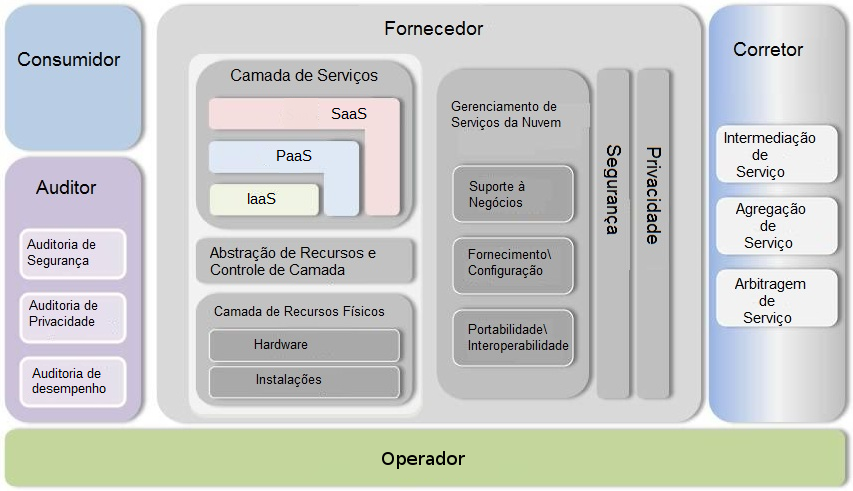
\includegraphics[width=0.8\textwidth]{img/nist_taxonomia.png}
	\label{fig:nist_taxonomy}\\
	Fonte: \cite{nist:modeloreferencia}.
\end{figure}

Segundo \cite{nist:modeloreferencia}, os principais atores envolvidos na computação em nuvem são definidos como:
\begin{itemize}
\item \textbf{Consumidor:} Uma pessoa ou organização que mantém uma relação de negócios com um \textit{Provedor} de serviços de nuvem, na qual utiliza o serviço oferecido pelo provedor.

\item \textbf{Provedor:} Uma pessoa, organização, ou entidade responsável por tornar o serviço de computação em nuvem disponível às partes interessadas.
%
As atribuições do \textit{Provedor} variam de acordo o tipo de serviço ofertado (\ac{iaas}, \ac{paas}, \ac{saas}), e são divididas com o \textit{Consumidor} conforme o tipo de serviço contratado.

\item \textbf{Auditor:} Uma pessoa ou entidade que conduz avaliações independentes de serviços de nuvem, e também de desempenho, segurança e operação de sistemas de informação presentes na implementação da nuvem.

\item \textbf{Corretor:} Entidade que controla o uso, desempenho e distribuição de serviços em nuvem, e intermedeia relações entre \textit{Provedor} e \textit{Consumidor}.
%
Este ator oferece um serviço que simplifica o acesso à diversos serviços de nuvem, como possibilitar, por exemplo, que o \textit{Consumidor} realize a integração entre serviços de nuvem sem necessitar que tenha conhecimento aprofundado;

\item \textbf{Operador:} Intermediário que provê conectividade e transporte de serviços de nuvem do \textit{Provedor} até o \textit{Consumidor}.
%
Ou seja, um ator neste caso pode ser uma companhia que oferece serviços de telecomunicação ou que transporta fisicamente dispositivos de armazenamento.
\end{itemize}

Para alguns destes atores, como o provedor e o auditor, há interesse em saber detalhadamente sobre a operação do serviço de computação em nuvem em questão.
%
Neste âmbito, a caracterização de tráfego oferece uma maneira de entender o que ocorre nas redes relacionadas à nuvem, permitindo entender mais detalhadamente o comportamento e desempenho da nuvem.
%
Com estas informações em mãos, torna-se possível por exemplo, descobrir o quanto é possível expandir a nuvem com a infraestrutura de rede atual, e também a entender como componentes internos da nuvem interferem no seu funcionamento.



Dentro dos modelos de serviços ofertados, este trabalho foca no tipo \ac{iaas}.
%
Neste sentido, usualmente os provedores \ac{iaas} fornecem serviços de virtualização, \textit{e.g.,} \ac{vm} e contêiner.
%
Os serviços baseados em \ac{vm} são os mais comumente ofertados e utilizados \cite{nicodemus:2016:conteineres}.
%
Segundo \citeonline{jain:2013:virtualizationsurvey}, a adoção de tecnologias de virtualização tem como um de seus principais motivos a facilidade de gerenciamento, obtida pela abstração dos recursos em função da virtualização.
%
Ou seja, os recursos computacionais são ofertados através de uma interface uniforme padronizada, que independente do hardware sendo virtualizado, os dispositivos virtuais funcionam da mesma maneira, o que simplifica seu uso e controle pelo consumidor ou provedor da nuvem.

%Apesar de impactante, a virtualização não é um conceito novo na computação.
%
%Memória foi o primeiro tipo de recurso a ser virtualizado, cujo uso de algoritmos de paginação permitiu otimizar o uso de um recurso tão caro na década de 1970 \cite{jain:2013:virtualizationsurvey}, que avançou, e atualmente disponibiliza, por exemplo, múltiplos níveis de \textit{cache} de memória.
%
%Consequentemente, a tecnologia passou a ser aplicada em diversos recursos computacionais, como armazenamento, rede e até o próprio processamento.


\subsection{Virtualização}

A virtualização é uma das tecnologias que servem como alicerce às nuvens computacionais.
%
Através da virtualização criam-se infraestruturas lógicas, incluindo topologias de redes e computadores, que funcionam sobre recursos físicos existentes.
%
Assim, possibilita-se criar, por exemplo, vários computadores virtuais, ou seja, \acp{vm}, que executam em apenas um computador físico, e contam com característica de isolamento, sendo controladas por algum software responsável (\textit{e.g.,} hipervisores, como: VirtualBox\footnote{\url{https://www.virtualbox.org}} e \ac{kvm}\footnote{\url{https://www.linux-kvm.org}}).

Segundo \citeonline{tanenbaum:2010}, a virtualização de redes computacionais pode ser feita através de uma \ac{vlan}, por exemplo, na qual um \textit{switch} com suporte a \ac{vlan} encaminha pacotes por suas diferentes portas em função da \ac{vlan} contida no cabeçalho de cada pacote, fornecendo a capacidade de isolamento entre computadores pertencentes à mesma rede física.
%
Em relação a comunicação das \acp{vm}, tecnologias de virtualização de rede instaladas num computador, como a \textit{Open vSwitch}\footnote{\url{http://openvswitch.org}} permite que \acp{vm} comuniquem-se através da Camada 2, independente da localização física da \ac{vm}, e também provê isolamento na comunicação das várias \acp{vm} executando em um computador \cite{callegati:2014:openstackVirtualization}.

Contudo, a virtualização adiciona camadas de abstração sobre a infraestrutura física existente, tal como o computador, por exemplo, que deve redirecionar e endereçar cada pacote na sua rede virtual. 
%
Outro ponto levantado por \citeonline{callegati:2014:openstackVirtualization} é referente ao monitoramento e controle de tráfego.
%
O tráfego entre \acp{vm} no mesmo computador não são comutados para a rede física, logo, não é possível empregar dispositivos para monitorar e filtrar pacotes de um jeito que não comprometa o isolamento e segurança da infraestrutura virtualizada.

A Figura~\ref{fig:openstack_network_adapter} ilustra a arquitetura de rede em um computador. 
%
Para um pacote originário da \texttt{vm01} alcançar a rede física (\texttt{vlan01}), é necessário que o pacote atravesse nove dispositivos virtuais no computador.
%
\pagebreak
\begin{figure}[!htb]
	\centering
	\caption{Redes virtualizadas em um computador.}
    \vspace{-0.3cm}
	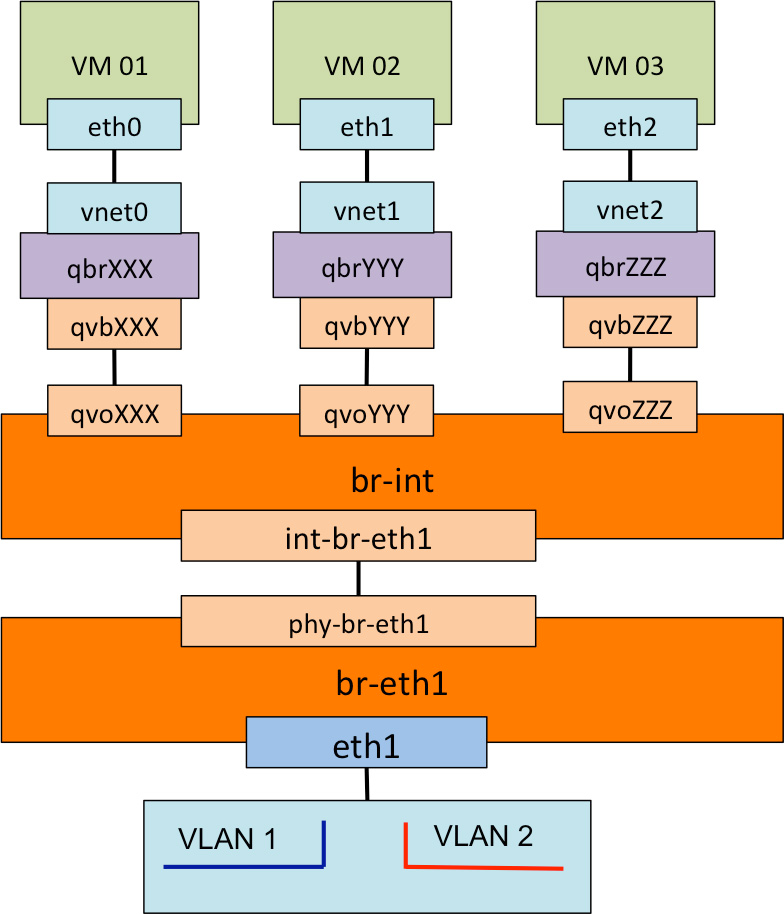
\includegraphics[width=0.5\textwidth]{img/openstack_virtualizacao.png}
	\label{fig:openstack_network_adapter}\\
    \vspace{-0.2cm}
	Fonte: \cite{zhang:2014:virtualizationtrafficanalysis}.
\end{figure}

Segundo \citeonline{zhang:2014:virtualizationtrafficanalysis}, dispositivos virtualizados \textit{Open vSwitch} presentes na Figura~\ref{fig:openstack_network_adapter} (\texttt{br-int, br-eth1}) comportam-se de maneira idêntica a \textit{switches} físicos.
%
Outros dispositivos virtualizados também estão presentes, como \textit{hubs} (\texttt{qbrXXX, qbrYYY, qbrZZZ}), e interfaces virtualizadas (\texttt{qvbXXX, qvoXXX, int-br-eth1}, e \texttt{phy-br-eth1}).
%
Ainda segundo \citeonline{zhang:2014:virtualizationtrafficanalysis}, a complexidade envolvida na transição dos pacotes entre as interfaces virtualizadas é significativa, e dificulta o processo de \textit{debugging} e correção de possíveis problemas.


Nuvens computacionais utilizam virtualização em todos os âmbitos discutidos simultaneamente, e necessitam de um software que gerencie o ciclo de vida e comunicação nestes ambientes.
%
Softwares que gerenciam nuvens computacionais possuem arquiteturas complexas em função da quantidade de tarefas que são responsáveis, tal como: balancear a carga entre os hosts, configuração, alocação e destruição de instâncias de \acp{vm}, gerenciar as imagens nas quais as \acp{vm} são armazenadas, gerenciar a conectividade de rede das \acp{vm}, disponibilizar interfaces para gerenciamento externo de \acp{vm}, etc.
%
A Seção~\ref{cap2:openstack} introduz os conceitos básicos sobre o software de gerenciamento de nuvem \ac{iaas} OpenStack\footnote{\url{https://www.openstack.org}}, que compõe o ambiente no qual planeja-se realizar a caracterização de tráfego, conforme proposto neste trabalho.
%
O OpenStack oferece serviços do tipo \ac{iaas}, podendo ser usado por um provedor para ofertar serviços tanto privados como públicos.

\section{OpenStack}
\label{cap2:openstack}

O OpenStack foi criado em 2010, através de uma colaboração entre a Rackspace e Anso Labs (contratada da NASA), o sistema está atualmente na sua 16\textsuperscript{a} versão, identificada pelo codinome ``Pike" \cite{openstack:about}.
%
\textbf{A versão do OpenStack abordada nesta seção é a Newton (2016)} para garantir que toda a discussão relacione-se com o ambiente no qual o trabalho está sendo realizado, que atualmente possui o OpenStack Newton instalado. 

O OpenStack permite controlar uma infraestrutura composta por recursos de computação, armazenamento e rede em um \textit{data center}.
%
O OpenStack possui diversas formas de acesso, sendo a mais básica através da interface web (Horizon) e as mais versáteis como \acp{api} que proporcionam acesso facilitado para os consumidores e provedores~\cite{openstack:about}. 

A principal forma de acesso é pela \ac{api}, que expõe funcionalidades da nuvem para serem acessadas por consumidores fisicamente distantes e por aplicações externas, permitindo por exemplo, a integração com outras nuvens.
%
Segundo ~\citeonline{corradi:2014:openstackConsolidation}, o serviço de \ac{api} do OpenStack é o seu \textit{front-end}, pois recebe requisições dos consumidores e as transforma em ações na nuvem.
%
As funcionalidades oferecidas desta maneira variam desde controle das \acp{vm} até autenticação.
%
Mais especificamente, a \ac{api} disponibiliza suas funcionalidades como \textit{Web Services}, cujas requisições são transportadas como mensagens HTTP com seu \textit{payload} em XML, que são interpretadas e convertidas para comandos na nuvem.
%
Através deste estilo de \textit{Web Service}, a \ac{api} do OpenStack fornece compatibilidade com nuvens de empresas distintas, como Eucalyptus e Amazon \cite{corradi:2014:openstackConsolidation}.


A instalação do OpenStack é modular, feita através de serviços, que para maior efetividade, funcionam sobre uma arquitetura recomendada de organização da rede.
%
\subsection{Serviços OpenStack}

A modularidade é um diferencial, pois permite acoplar serviços para adicionar funcionalidades extras a uma instalação existente, como serviço de banco de dados (\textit{e.g.,} Trove).
%
De acordo com \citeonline{Litvinski:2013:openstackmodules}, esta arquitetura modular independente e com comunicação assíncrona foi criada para garantir a elasticidade e escalabilidade horizontal, na qual serviços podem ser utilizados em qualquer instalação.
%
A Tabela~\ref{tab:openstack_service_list} contém alguns dos serviços de uma instalação de exemplo do OpenStack Newton, segundo a documentação do projeto \cite{openstack:newton}.

\begin{table}[!htb]
\centering
\scriptsize
\caption{Lista de serviços em uma instalação básica do OpenStack}
\begin{tabularx}{1\textwidth}{lllX}
\hline
\textbf{\begin{tabular}[c]{@{}l@{}}Tipo de \\ serviço\end{tabular}}      & \textbf{\begin{tabular}[c]{@{}l@{}}Nome do\\ serviço\end{tabular}} & \textbf{Portas (TCP)}                                                     & \textbf{Descrição}                                                                                                                                                                \\ \hline
Dashboard                                                                & Horizon                                                            & 80, 443                                                             & Disponibiliza uma interface gráfica web para interagir com serviços subjacentes do OpenStack (e.g., iniciar uma instância, atribuir endereços IP, e definir permissões de acesso) \\
\rowcolor[HTML]{EFEFEF} 
Computação                                                               & Nova                                                               & \begin{tabular}[c]{@{}l@{}}8773 - 8775, \\ 6080 - 6082\end{tabular} & Gerencia o ciclo de vida de instâncias de processamento em um ambiente OpenStack. Responsabilidades incluem iniciação, escalonamento e desalocação de VMs de acordo com a demanda \\
Rede                                                                     & Neutron                                                            & 9696                                                                & Habilita o serviço de conectividade de rede para outros serviços OpenStack, como o Nova. Provê uma API para consumidores definirem as redes e suas particularidades                   \\
\rowcolor[HTML]{EFEFEF} 
\begin{tabular}[c]{@{}l@{}}Armazenamento\\ de objeto\end{tabular}        & Swift                                                              & \begin{tabular}[c]{@{}l@{}}6000 - 6002,\\ 873\end{tabular}          & Armazena e recupera objetos contendo dados não estruturados através de sua API. Possui tolerância a falha através da replicação de dados numa arquitetura espalhada/horizontal    \\
\begin{tabular}[c]{@{}l@{}}Armazenamento\\ de bloco para VM\end{tabular} & Cinder                                                             & 8776, 3260                                                          & Disponibiliza armazenamento persistente em bloco para instâncias em execução                                                                                                      \\
\rowcolor[HTML]{EFEFEF} 
Identificação                                                            & Keystone                                                           & 5000, 35357                                                         & Disponibiliza um serviço de autenticação e autorização para outros serviços do OpenStack. Inclui autenticação da API e descoberta de serviços                                     \\
Imagem de VM                                                             & Glance                                                             & 9292, 9191                                                          & Armazena e recupera as imagens utilizadas nas VMs. O serviço Nova utiliza este serviço durante o provisionamento de instância de VMs                                              \\
\rowcolor[HTML]{EFEFEF} 
Telemetria                                                               & Ceilometer                                                         & 8777                                                                & Monitora e mede o uso da nuvem para cobrança, benchmark e outros fins estatísticos                                                                                                \\ \hline
\end{tabularx}
\label{tab:openstack_service_list}\\
Fonte: Adaptado de \cite{openstack:newton}.
\end{table}


Na Tabela~\ref{tab:openstack_service_list}, o único serviço não presente nesta lista em relação à documentação é o Heat, que é um serviço opcional, responsável por orquestrar e sincronizar múltiplas nuvens.
%
Para os serviços funcionarem corretamente as portas listadas nesta tabela, que utilizam TCP, não podem ser bloqueadas pelos \textit{firewalls} pertencentes à infraestrutura da nuvem.
%
Além destas portas, existem outras portas TCP de propósito geral no OpenStack, como a TCP/3306 (acesso ao MySQL), que é utilizada pela maioria dos serviços, e a porta TCP/5672, na qual o RabbitMQ, um servidor para troca de mensagens \ac{amqp} opera, e é responsável pela comunicação interna dos serviços Nova, Neutron e Cinder (explicado na Seção~\ref{cap3:openstack_detalhes}).

A Figura~\ref{fig:openstack_service_architecture} ilustra como serviços básicos do OpenStack se relacionam.
%
Nos serviços de alto nível, há relacionamento direto com múltiplos serviços, tanto para disponibilizar funcionalidades para outros serviços (\textit{e.g.,} Keystone), quanto para utilizar ou acessar recursos de outros serviços (\textit{e.g.,} Horizon e Ceilometer, respectivamente).
%
O Keystone cuida da autenticação e autorização dentro da nuvem, que é consultado pelos serviços da nuvem antes de executar alguma ação solicitada pela \ac{api}, por exemplo, com o objetivo de confirmar a identidade do solicitante.
%
O objetivo do Horizon é disponibilizar uma interface gráfica (\textit{front-end}), que possibilita ao consumidor gerenciar, criar e iniciar suas instâncias e respectivas configurações (\textit{e.g.,} rede, sistema operacional e características físicas (\textit{flavor})), que então são transformadas em chamadas de \ac{api} e enviadas para outros serviços do OpenStack.
%
O Ceilometer é o serviço que monitora e analisa o desempenho do OpenStack, disponibilizando métricas relacionadas a rede (\textit{e.g.,} quantia de bytes enviado por cada interface, quantia de erros de envio e recebimento por interface),  armazenamento (\textit{e.g.,} tamanho de imagem, latência do armazenamento de instância), processamento (\textit{e.g.,} uso de memória de instância, quantia de instruções executadas), entre outros, que podem ser empregadas para \textit{benchmark} ou cobrança pelo uso dos recursos, por exemplo.

\begin{figure}[!htb]
	\centering
	\caption{Arquitetura conceitual entre serviços do OpenStack}
	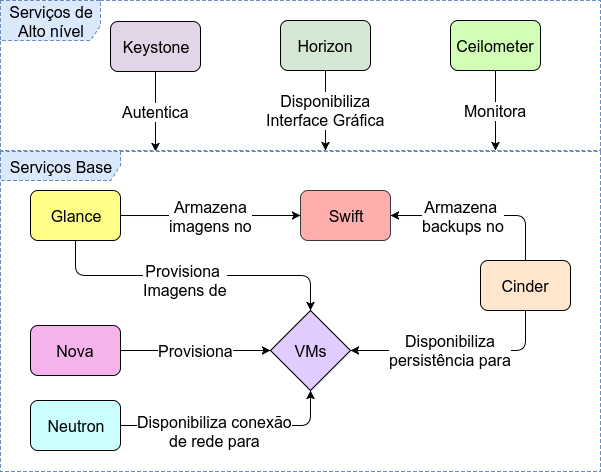
\includegraphics[width=0.8\textwidth]{img/openstack_arquitetura_servicos.png}
	\label{fig:openstack_service_architecture}\\
	Fonte: Adaptado de \cite{openstack:newton}.
	%https://docs.openstack.org/newton/install-guide-debconf/common/get-started-conceptual-architecture.html
\end{figure}

Em relação aos serviços base, segundo \citeonline{openstack:newton}, a maioria está relacionado com disponibilizar funcionalidades para instâncias (representado na Figura \ref{fig:openstack_service_architecture} pelo losângulo escrito \acp{vm}, na qual apenas o Swift não tem relação direta), e neste sentido, segundo \citeonline{kumar:2014:openstackarchitecture}, para manter a modularidade e consequentemente a escalabilidade, o OpenStack divide responsabilidades sobre múltiplos serviços, como por exemplo, o Glance armazenar no Swift as imagens de sistemas operacionais que disponibiliza.
%
O Nova, por exemplo, utiliza múltiplos serviços durante certas tarefas, como no provisionamento de instância de \ac{vm}, na qual requisita a imagem do sistema operacional ao Glance, configura a rede da instância com o Neutron e disponibiliza armazenamento persistente para a instância através do Cinder.




A instalação destes serviços nos servidores também pode seguir uma arquitetura sugerida.
%
Segundo o \citeonline{openstack:newton}, uma instalação adequada do OpenStack contém vários computadores que hospedam serviços (hosts), que são divididos em pelo menos dois tipos: controle e computação.
%
Ao longo deste trabalho, ao referenciar-se um host com papel específico em uma nuvem (\textit{e.g.,} controle, computação), este será chamado por nó, seguido do seu papel (\textit{e.g.,} nó de controle, nó de computação). 
%
Dentro de uma nuvem podem haver múltiplos hosts distribuídos entre computação e controle, na qual nós de controle executam serviços que gerenciam e dispõem recursos à nuvem, enquanto que nós de computação hospedam instâncias.
%
Caso sejam adotados os serviços na Figura \ref{fig:openstack_service_architecture}, por exemplo, todos os serviços, menos parte do serviço Nova ficariam hospedados em nós de controle.
%
Isto ocorre pois de acordo com \citeonline{corradi:2014:openstackConsolidation}, o Nova divide-se em quatro componentes: \ac{api}, computação, escalonador, e o gerenciador de rede, que foi substituído pelo Neutron.
%
O serviço de \ac{api} do Nova é responsável por disponibilizar acesso e controle às instâncias, tanto internamente quanto por acesso externo.
%
O serviço de computação é instalado nos nós de computação, e é quem se comunica com o software gerenciador de \acp{vm} (\textit{hypervisor}), também instalado em cada nó de computação.
%
Dentre as responsabilidades do serviço de computação está gerenciar o ciclo de vida das instâncias e acessar métricas de desempenho e carga do \textit{hypervisor}.
%
O serviço de escalonamento recebe os pedidos de instância de \ac{vm} pela \ac{api}, e então realiza o escalonamento para decidir em qual nó de computação a instância será alocada.

É possível executar todos estes serviços em um mesmo host, contudo, não há necessidade, pois é possível empregar apenas um nó controlador para inúmeros nós de computação.
%
Também podem ser adicionados nós de controle redundantes, que realizam as mesmas tarefas e estão sempre em sincronia, e garantem, portanto, o funcionamento ininterrupto da nuvem caso um dos nós de controle fique indisponível.
%
Esta comunicação entre nós de controle e computação ocorre na rede de controle, contida no Domínio de Controle, apresentado na Seção \ref{cap2:openstack_network_architecture}.
%
Considerando as diversas possibilidades de instalação de uma nuvem OpenStack, sua documentação define uma organização básica da rede, que possibilita escalar a nuvem e seus serviços.

\subsection{Arquitetura de rede}
\label{cap2:openstack_network_architecture}

Para realizar a comunicação entre os host que hospedam diferentes serviços são utilizadas redes físicas de acordo com infraestrutura recomendada, conforme ilustrado na Figura~\ref{fig:openstack_network_architecture}. 
%
Esta arquitetura possui três domínios com políticas de seguranças distintas: Domínio Público, Domínio de Controle e Domínio de Convidados \cite{openstack:newton}. 
%
Os três domínios englobam quatro redes distintas, cujas políticas de segurança das redes correspondem ao domínio na qual pertencem, e são divididas em -- \textbf{Domínio Público}: rede externa e rede de \ac{api}; \textbf{Domínio de Convidados}: rede de convidados; e \textbf{Domínio de Controle}: rede de controle e rede de armazenamento (opcional).

\vspace{-0.4cm}
\begin{figure}[!htb]
	\centering
	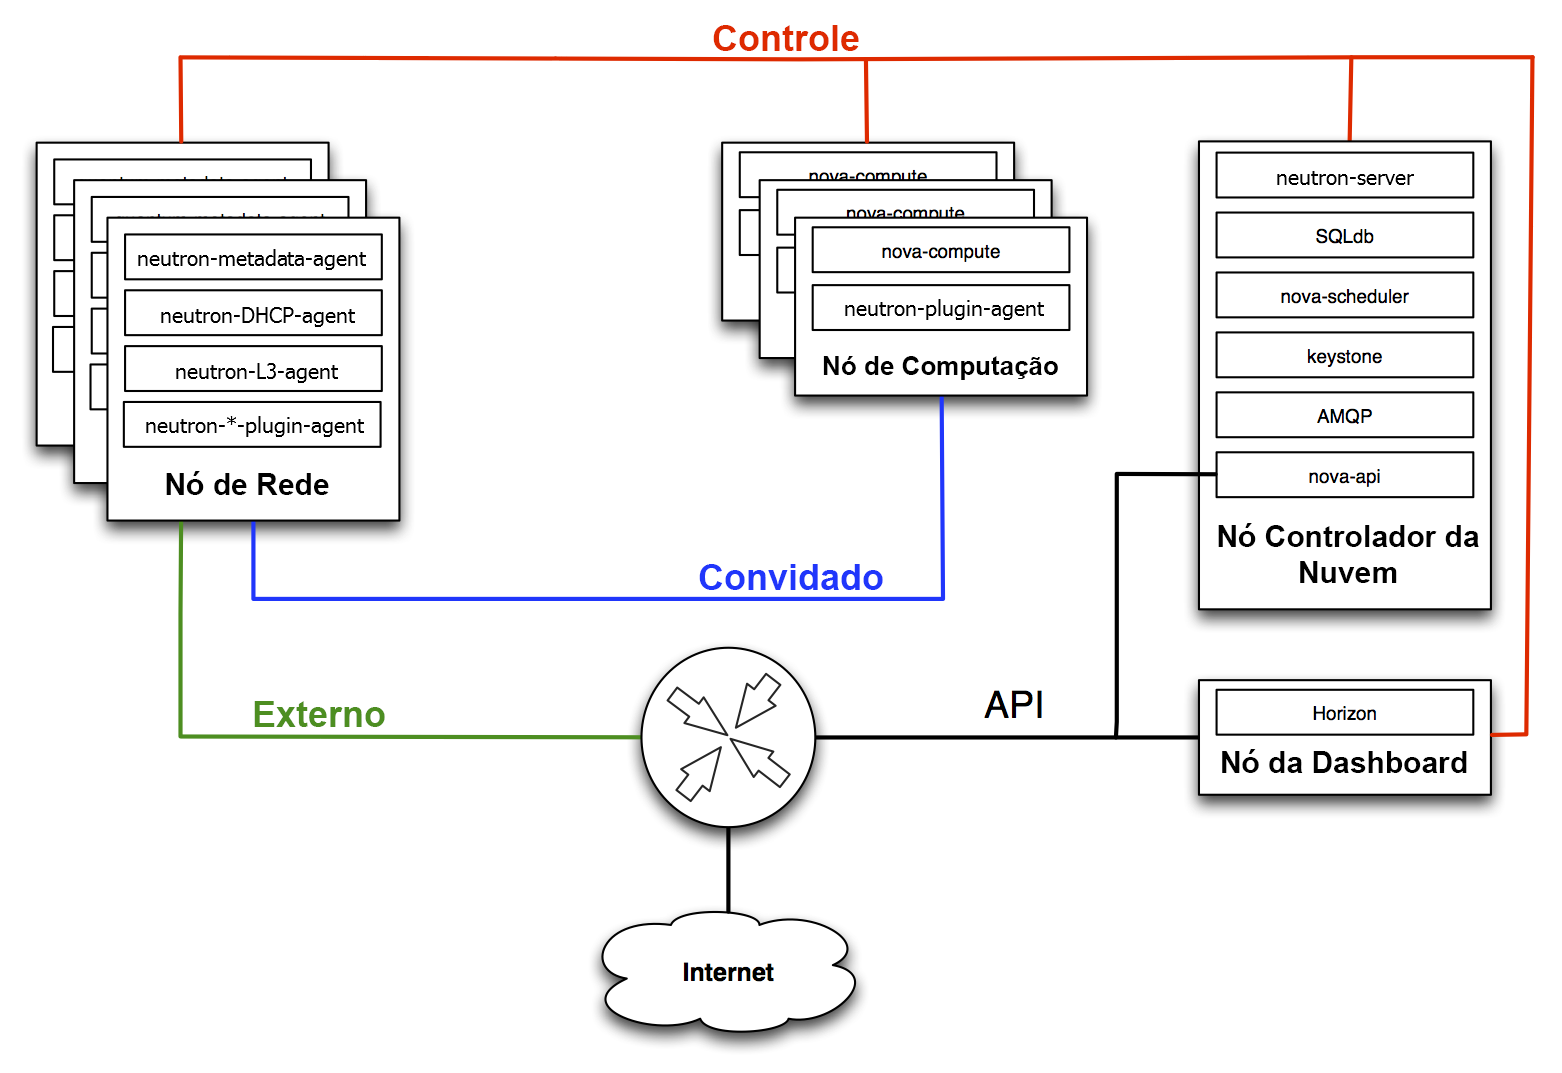
\includegraphics[width=0.8\textwidth]{img/openstack_arquitetura_rede.png}
    \vspace{-0.3cm}
	\caption{Arquitetura de rede física recomendada para o OpenStack}
	\label{fig:openstack_network_architecture}
	Fonte: Adaptado de \cite{openstack:networkguide}
\end{figure}

O \textbf{Domínio Público} envolve as redes responsáveis pela visibilidade da \ac{api} da nuvem criada na Internet e do acesso à Internet pelas \acp{vm}, que correspondem respectivamente à rede externa e à rede de \ac{api}.
%
Em ambas as redes, todos os endereços IPs devem ser visíveis a partir da Internet para seu pleno funcionamento.

No \textbf{Domínio de Convidados} encontra-se a rede responsável pela comunicação entre as \acp{vm}. 
%
Os consumidores do serviço de oferta de \acp{vm} são referenciados como convidados por não possuírem vínculo direto com a administração da nuvem, logo, não há garantias sobre quem estes convidados são e quais os seus objetivos.
%
Portanto, tecnologias de virtualização da rede são empregadas em cada nó de computação para isolar o tráfego de cada \ac{vm} e impedir que elas sejam capazes de interferir ou visualizar o tráfego para as outras \acp{vm} no mesmo host. 
%
Mais especificamente, o serviço Neutron é responsável pela virtualização de rede de convidado, na qual permite \textit{multitenancy} através de \textit{network namespaces}.
%
\textit{Multitenancy} é uma arquitetura de software que permite isolar um grupos de consumidores da nuvem (\textit{tenant} ou \textit{project} em versões mais recentes do OpenStack) de maneira que eles compartilhem o acesso a certos recursos, cada qual com privilégios específicos.
%
Ou seja, é possível permitir que certas \acp{vm} criem redes virtuais entre si como se fizessem parte da mesma rede física, e portanto, podem comunicar-se diretamente, isso tudo de acordo com a configuração dos consumidores.
%
Segundo \cite{denton:2016:neutron}, um \textit{network namespace} é definido como uma cópia lógica de uma rede, com regras de roteamento e \textit{firewall} próprias e dispositivos de interface de rede virtuais.
%
O Neutron provê DHCP e roteamento próprio para cada \textit{namespace} e permite que a rede de um \textit{project}/\textit{tenant} conecte-se com o Domínio Público (Internet) adicionando um roteador virtual à sua rede.

O \textbf{Domínio de Controle} contém a rede responsável pelo tráfego de controle e de armazenamento do OpenStack, que corresponde ao tráfego gerado pela comunicação entre os seus serviços. 
%
Esta rede é um ambiente acessível apenas pelo software que gerencia a nuvem, e apenas os administradores da nuvem tem a capacidade de acessá-la em condições normais, dispensando a necessidade de isolamento através da virtualização.
%
Neste sentido, a virtualização de rede está presente apenas nos nós de computação, que virtualizam todas as interfaces de rede em conjunto com o \textit{hypervisor}.
%
Tanto os nós controladores da nuvem quanto os de computação têm interfaces físicas que ligam-se à rede de controle, e portanto, a documentação do OpenStack recomenda que todos os nós pertencentes à nuvem possuam duas interfaces de rede cada.
%
Múltiplas interfaces de rede física permitem conectividade à rede de controle e a outras redes conforme o caso, como a rede de convidados no caso de nós de computação, ou a rede pública no host responsável por gerenciar a rede das \acp{vm}.
%
Portanto, uma \ac{vm} em execução só poderá acessar a rede de controle caso consiga executar um ataque de elevação de privilégio e tenha acesso às interfaces de rede físicas do host na qual a \ac{vm} em questão está alocada \cite{Krutz:2010:cloudsecurity}.

Para exemplificar o funcionamento da rede de controle, a Figura \ref{fig:openstack_criacao_instancia} ilustra o processo de criação de instâncias do OpenStack do ponto de vista dos serviços, em alto nível.
%
A comunicação entre os serviços é realizada através da rede de controle, ou seja, todas as setas na figura representam tráfego gerado na rede durante o processo.
%
Opcionalmente, é possível criar uma rede de transferência de arquivos, separada da rede de controle, mas contida no Domínio de Controle, com o objetivo de otimizar o uso de banda para serviços relacionados com transferência de arquivos (Swift, Cinder), que podem ser responsáveis por boa parte do tráfego de controle.

\begin{figure}[!htb]
	\centering
	\caption{Diagrama de sequência em alto nível: Criação de instância no OpenStack}
	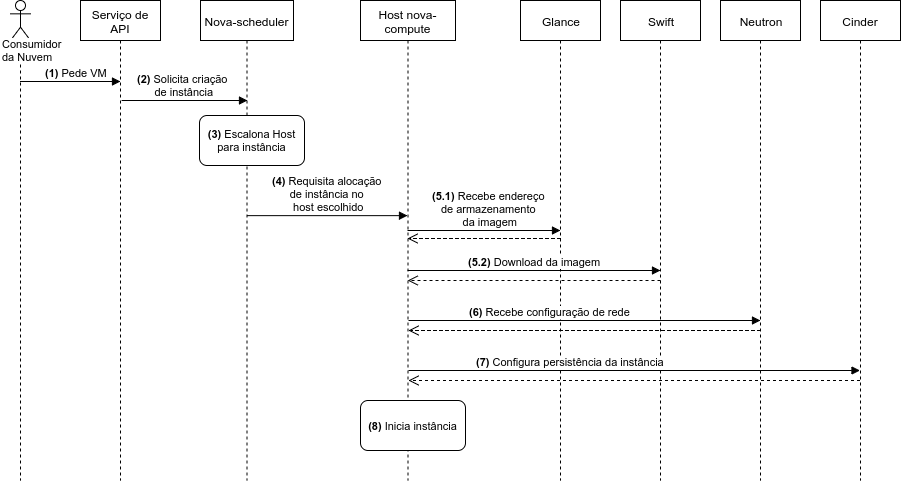
\includegraphics[width=1\textwidth]{img/openstack_criacao_instancia.png}
	\label{fig:openstack_criacao_instancia}\\
	Fonte: O próprio autor.
\end{figure}

\begin{enumerate}[label*=\arabic*.]
\item O processo de criação de instância inicia com um pedido de \ac{vm} por um consumidor da nuvem através da interface gráfica no Horizon, que realiza o pedido na \ac{api}, ou diretamente pela \ac{api}.
%
Para simplificar o diagrama, o serviço Keystone foi omitido, e sua responsabilidade está relacionada com esta etapa \textbf{(1)}, cuja \ac{api} autentica o consumidor da nuvem para garantir que ele possui as permissões necessárias;
%
\item A \ac{api} então comunica o serviço Nova-scheduler, responsável pelo escalonamento;

\item O componente Nova-scheduler, que executa em um nó de controle define em qual nó de computação a instância será executada; 

\item Após realizar o escalonamento, repassa o pedido para o nó de computação escolhido. O nó de computação recebe o pedido de instância, que contém informações como imagem a ser utilizada na \ac{vm} (\textit{flavor}), e as características da \ac{vm} (\textit{e.g.,} memória, processamento, rede), e inicia o processo de configuração da instância de \ac{vm};

\item O processo para recuperar a imagem do sistema operacional a ser utilizada na \ac{vm} é divido em dois passos;

\begin{enumerate}[label*=\arabic*.]

\item O primeiro passo corresponde à buscar o endereço de armazenamento da imagem no Glance; e

\item Então, no segundo passo, recupera do Swift o dado não estruturado que contém a imagem correspondente. Após recuperada a imagem, os passos posteriores no processo são responsáveis por configurar o ambiente na qual a \ac{vm} executará, e a ordem que ocorre pode não ser a mesma deste diagrama de sequência;

\end{enumerate}

\item A configuração da rede da \ac{vm} é fornecido pelo Neutron, que define as configurações de acordo com o \textit{tenant} e realiza as modificações necessárias na rede.
%
\item A última configuração necessária é a persistência de dados da \ac{vm}, que é fornecido pelo Cinder, serviço responsável pelo armazenamento de bloco.
%
\item Com todas as configurações definidas, o passo final é a inicialização da \ac{vm} pelo nó de computação que hospedará a instância.
\end{enumerate}

Nota-se que o OpenStack possui vários serviços que podem estar dispostos em hosts distintos. 
%
Nesse sentido, o tráfego do Domínio Público reflete o tráfego normal das aplicações hospedadas.
%
Em contrapartida, o tráfego do Domínio de Controle e Domínio de Convidado são transações internas da nuvem, às quais não são visíveis a perspectiva do consumidor.
%
Ou seja, esse tráfego possui características intrínsecas à solução de nuvem e à sua arquitetura de implantação.
%
O foco deste trabalho é caracterizar o tráfego do Domínio de Controle para levantar aspectos operacionais e de desempenho de uma nuvem OpenStack.

\section{Caracterização de Tráfego}
\label{cap2:caracterizacao}

A medição / caracterização do tráfego é uma tarefa empregada para entender e resolver problemas relacionados com o desempenho em redes de computadores ~\cite{dainotti:2006:packetcharacterization}. 
%
Pretende-se ter a caracterização de tráfego neste trabalho como fim, ou seja, a rede caracterizada será o produto da aplicação de técnicas que analisam o tráfego e de análises posteriores dos dados gerados.
%
O processo de caracterização de tráfego é descrito nesta seção em duas etapas: medição de tráfego/levantamento de dados e a análise do tráfego obtido.
%

\subsection{Medição de Tráfego}

Durante a medição de tráfego, são capturados os dados que trafegam pela rede da qual pretende-se caracterizar o tráfego.
%
Na captura dos dados são utilizadas ferramentas (\textit{e.g.,} tcpdump) que realizam a captura dos dados através de duas abordagens: medição ativa e medição passiva.
%
Após a captura, o tráfego então é abstraído em um certo nível de agregação (\textit{e.g.,} fluxo, pacote e bytes), variando de acordo com as capacidades da ferramenta de monitoramento e a técnica de análise empregada  ~\cite{dainotti:2006:packetcharacterization}.

\subsubsection{Tipo de Medição}

Atualmente existem duas abordagens para realização de medição do tráfego de rede: medição ativa e medição passiva \cite{vilela:2006:caracterizacao, williamson:2001:internet}.
%
A medição ativa injeta tráfego na rede e mede o seu desempenho baseado no que foi injetado.
%
Este tipo de medição é considerado intrusivo, pois o processo gera tráfego, que influencia no funcionamento da rede, e consequentemente na medição.
%
Desta forma, medições ativas requerem cuidados na utilização, pois deve ser levado em consideração o tráfego gerado pela medição na etapa de análise do tráfego, posteriormente.
%
Ao medir o comportamento de filas em um roteador, por exemplo, o processo de medição pode alterar o comportamento da fila e influenciar nos resultados~\cite{vilela:2006:caracterizacao}.
%
De acordo com \citeonline{williamson:2001:internet}, algumas ferramentas para medição ativa são: \texttt{ping}, \texttt{traceroute} e \texttt{pathchar}. O \texttt{ping} fornece a latência na rede até um certo destino, \texttt{traceroute} fornece o caminho pelo qual um pacote foi roteado até o seu destino, e o \texttt{pathchar} estima o uso de banda e latência dos nós até um destino.

Por outro lado, a medição de tráfego passiva é usada para observar e armazenar o tráfego de pacotes em uma rede sem injetar qualquer tráfego na rede durante o processo de medição.
%
Ou seja, a medição de tráfego é não intrusiva~\cite{williamson:2001:internet}.
%
Neste sentido, a medição passiva necessita que sejam criados pontos de monitoramento por onde deseja-se coletar o tráfego, seja ele por hardware específico, ou dispositivos que pertençam a topologia e disponham desta funcionalidade~\cite{vilela:2006:caracterizacao}.
%
O protocolo \ac{snmp}, presente em vários dispositivos de rede permite o monitoramento de variáveis relacionadas ao tráfego (\textit{e.g.,} utilização de banda, perda de pacote) e do dispositivo (\textit{e.g.,} uso de processador e memória)~\cite{grossglauser:2002:snmp}.
%
Ainda segundo \citeonline{grossglauser:2002:snmp}, estes dados disponibilizados pelos dispositivos através do \ac{snmp} são acessados e armazenados por um software que monitora e gerencia a rede.
%
Contudo, estes dados não relevam detalhes suficientes para detectar a origem de um problema na rede (\textit{e.g.,} \ac{ddos}), necessitando a coleta de tráfego para obter-se maiores detalhes.
%
A coleta de tráfego em dispositivos de rede pode ser realizada utilizando protocolos implementados com este fim, que dentre as ferramentas existentes destacam-se: NetFlow e sFlow.
%
A ferramenta NetFlow, presente em roteadores da marca Cisco disponibiliza a medição passiva de tráfego TCP e UDP, agregando-o em fluxos \cite{vilela:2006:caracterizacao}.
%
sFlow foi criado através de um consórcio entre várias empresas (\textit{e.g.,} HP, Hitachi, Brocade, etc), com o objetivo de criar uma ferramenta escalável de coleta de tráfego.
%
A ferramenta sFlow funciona de maneira similar à Netflow, agregando os pacotes em fluxos, mas aplicando obrigatoriamente a técnica de amostragem sistemática, apresentada na Seção \ref{cap2:agregacao_trafego}, com o objetivo de alcançar escalabilidade com monitoramento em tempo real \cite{sflow:2003}.


\subsubsection{Nível de agregação do tráfego}
\label{cap2:agregacao_trafego}

O nível de agregação do tráfego define a granularidade dos dados a serem trabalhados, ou seja, o quão detalhada é a representação do tráfego.
%
Portanto, uma caracterização de tráfego com alto nível de granularidade (fino), por exemplo, exigirá uma quantidade maior de armazenamento e processamento posteriormente, mas com a vantagem de representar o tráfego com alta fidelidade.

Contudo, deve-se levar em conta a abordagem que será utilizada na etapa de análise do tráfego ao decidir a granularidade, pois os dados coletados servirão como entrada para abordagem escolhida.
%
Neste sentido, por exemplo, algumas técnicas de análise utilizam apenas informações contidas no cabeçalho dos pacotes, descartando-se o \textit{payload}.
%
Ao empregar técnicas deste tipo não há ganho em representar o tráfego com uma granularidade fina, em função da alta quantidade de armazenamento e tempo de processamento necessários.
%
Segundo a taxonomia de \citeonline{khalife:2014:taxonomy}, o tráfego é comumente agregado nos seguintes níveis:

\begin{itemize}
	\item \textbf{Pacote:} Todos os pacotes que trafegam na rede são armazenados, e é um nível de agregação com granularidade fina, ou seja, com maior quantidade de dados.
	%
	Neste nível, exemplos de dados coletados são IP de origem e destino, tamanho do pacotes, números do protocolo e \textit{payload}.
	%
	Ferramentas como TCPdump\footnote{\url{http://www.tcpdump.org}} e SNORT\footnote{\url{https://www.snort.org}} são capazes de fazer captura neste nível \cite{callado:2009:survey}.
	
	\item \textbf{Fluxo:} Agregação de pacotes em um único objeto, obtido através da aplicação de uma regra de agregação durante a medição do tráfego, como por exemplo, agrupar pacotes com mesma porta e IP de origem e destino, e portanto, possui granularidade maior que o pacote.
	%
	Os dados coletados nesse nível são: fluxos por unidade de tempo, tamanho do fluxo, duração do fluxo \cite{callado:2009:survey}. 
	%
	Ferramentas como Cisco NetFlow e sFlow são comumente utilizadas para coleta neste nível.
	
	\item \textbf{Host:} Agregação com granularidade grossa, na qual um host é um objeto, representado pelo seu respectivo endereço IP.
	%
	Neste nível, é associado o uso de uma aplicação a um host, e portanto a quantidade de dados é limitada.
	%
	Um exemplo é o Blinc, criado por \citeonline{Karagiannis:2005:Blinc}, que analisa as interações do host num alto nível, como o seu papel na rede baseado na quantidade de portas (atua como provedor de algum serviço) e sua interação com outros host (popularidade na rede).
\end{itemize}

Dentre os níveis de agregação de tráfego apresentados, segundo ~\citeonline{khalife:2014:taxonomy}, a agregação por fluxo foi o mais adotado nos trabalhos analisados.
%
Isto pode estar relacionado com a similaridade nas informações disponíveis nos níveis de fluxo e pacote, e também, em certas situações a análise com granularidade fina é impraticável por conta da quantidade de tráfego gerado (\textit{e.g.,} \textit{data centers} e \textit{backbones}), cuja utilização de fluxos é viável.

De acordo com \citeonline{callado:2009:survey}, durante o processo de medição de tráfego é possível compactar a quantidade de dados gerados com qualquer granularidade através do emprego de técnicas de amostragem.
%
Ainda segundo \citeonline{callado:2009:survey}, esta fase opcional é disponibilizada pelo processo de amostragem sistemática em alguns roteadores da Cisco na funcionalidade de coleta de pacotes.
%
A amostragem sistemática, representada pela expressão $\frac{1}{n}$, significa que nestes casos haverá a coleta apenas do 1\textsuperscript{o} pacote a cada $n$ pacotes.
%
Apesar de parecer questionável quando aplicado a situações com grandes variações, um dos estudos levantados pelo autor indicou que não há uma perda de precisão relevante no processo, e a amostragem permitiu uma significativa redução do uso do processador e rede pelo roteador.

\subsection{Análise de Tráfego}

A etapa posterior à medição do tráfego é a de análise do tráfego, em que todo o tráfego coletado é analisado.
%
Não foi identificado um método específico para realizar a caracterização de tráfego.
%
Portanto, nesta etapa são apresentadas técnicas de classificação com maior abrangência, que podem ser utilizadas, por exemplo, para classificação e análise de tráfego em tempo real.
%
As técnicas de classificação categorizam o tráfego em função da correspondência de características presentes no tráfego obtido com suas respectivas classificações. 
%
Segundo a taxonomia de \citeonline{khalife:2014:taxonomy}, as técnicas de classificação são divididas em inspeção de conteúdo, análise de características do tráfego ou abordagens híbridas entre elas.

As primeiras técnicas a surgirem baseavam-se apenas na inspeção do conteúdo de pacote, em que comparam o conteúdo do tráfego na rede com amostras já classificadas. 
%
Um arquivo de vídeo sendo transmitido na rede, por exemplo, pode ser detectado pela presença de uma sequência de bytes característicos, ou seja, sua assinatura~\cite{dharmapurikar:2003:bloomfilters}. 
%
A verificação de assinatura é efetuada através da busca por sequências de bytes idênticas, ou a avaliação com expressões regulares.
%
Contudo, limitações com questões de privacidade, a popularização da criptografia e a quantidade de processamento necessário limitam sua efetividade~\cite{park:2011:finegrained}.

A análise de características de tráfego é complementar à inspeção do conteúdo, na qual classifica o tráfego através das informações do cabeçalho e metadados relacionados ao tráfego analisado.
%
Essa análise também é conhecida como classificação às escuras, e resulta na criação de perfis de tráfego e a sua consequente análise estatística.
%
As técnicas de análise de características de tráfego utilizam abordagens gráficas ou estatísticas, que subdividem-se em modelos estatísticos simples ou com auxílio de \textit{machine learning}. 
%
As principais  técnicas que analisam características do tráfego são:
	
\begin{itemize}
	\item \textbf{Gráfica: }Técnicas gráficas, como em \citeonline{edward:2009:motif}, ilustram as interações entre os computadores em uma rede através de grafos baseados no tráfego analisado. 
	%
	Nesta representação os nós são os hosts envolvidos e as arestas a interação entre eles. 
	%
	Esta modelagem baseia-se na ideia que hosts envolvidos na mesma aplicação apresentam padrões que revelam tal comportamento, ao mesmo passo que a utilização de grafos facilita a visualização destes padrões.
	
	\item \textbf{Modelagem estatística simples: }Técnicas nesta categoria analisam atributos genéricos do tráfego e suas respectivas correlações estatísticas para identificar as aplicações executando no tráfego analisado. 
	%
	O princípio base desta abordagem é de que o tráfego na camada de rede possui propriedades estatísticas (\textit{e.g.,} distribuição do tamanho dos pacotes, tempo entre seus recebimentos) que são únicos para certas classes de aplicações, permitindo sua distinção \cite{nguyen:2008:machinelearningsurvey}. 
	%
	A utilização de heurísticas, por exemplo, estende esta abordagem aplicando um conjunto de regras baseados nas informações processadas \cite{Karagiannis:2005:Blinc}. 
	%
	Outra extensão é com a análise de perfil, que avalia o nível de heterogeneidade de um comportamento em relação ao perfil de tráfego comum àquela rede \cite{xu:2005:backboneprofiling}.
	
	\item{\textbf{Estatística com machine learning: }}De acordo com \citeonline{williams:2006:machinelearningcomparison}, algoritmos de \textit{machine learning} comparam tráfego com os mesmos conjuntos de características, procurando semelhanças para agrupá-los em \textit{clusters}. 
	%
	As duas principais abordagens na caracterização de tráfego são \textit{machine learning} não supervisionado e \textit{machine learning} supervisionado.
	%
	Técnicas com \textit{machine learning} supervisionado fornecem um conjunto de tráfego pré classificado, na qual o algoritmo analisa e treina para descobrir as prováveis correlações. 
    %
    Então, é aplicado a sua análise no conjunto de tráfego a ser classificado, que deve possuir as mesmas características observáveis do conjunto de treino.
	%
	No \textit{machine learning} não supervisionado é dado como entrada um conjunto de tráfego sem nenhuma classificação prévia, o algoritmo representa estes tráfegos de alguma forma, com vetores, por exemplo, e utiliza algum método de comparação, como a distância Euclidiana para verificar sua similaridade e agrupá-los~\cite{williams:2006:machinelearningcomparison}.	
\end{itemize}

Em relação às abordagens de análise apresentadas, a de análise estatística simples possui maior aplicabilidade, pois qualquer ambiente que gere métricas quantitativas pode empregá-lo.
%
Por exemplo, dos trabalhos relacionados apresentados na Seção \ref{cap2:relacionados}, três deles utilizam a análise estatística simples \cite{Sciammarella:2016:controltraffic, Wang:2010:ec2networkperformance, venzano:2013:trafficprivatecloud}, enquanto apenas um aplica a abordagem gráfica \cite{sharma:2015:hansel}.
%
Para a caracterização proposta neste TCC, a análise estatística simples inicialmente apresenta maior versatilidade, podendo ser mais facilmente adequada conforme define-se os detalhes da caracterização do tráfego.
%
Assim, como as métricas em sua maioria relacionam-se com desempenho, na fase de análise do tráfego, esta  técnica inicialmente possui o potencial de fornecer bons resultados ao mesmo passo que possui baixa complexidade.

No geral, as abordagens de análise apresentadas (estatística simples, gráfica, estatística com \textit{machine learning}) têm foco na análise das características presentes no tráfego, na qual empregam características comuns a qualquer tipo de tráfego, ou seja, aplicáveis para analisar qualquer tráfego.
%
Contudo, em certas situações, é possível utilizar informações relacionadas à rede na qual planeja-se caracterizar o tráfego para diminuir a complexidade na etapa de medição e análise de tráfego.
%
Informações sobre protocolos de aplicação em execução na rede, por exemplo, facilitam a identificação do comportamento do tráfego, e a identificar qual parte dele fornecerá resultados relevantes.
%
Neste sentido, sua aplicabilidade é limitada a redes cujo comportamento seja previsível.
%
Segundo \citeonline{karagiannis:2004:p2p}, por exemplo, monitorar aplicações apenas em função das portas e protocolos padrões não apresenta resultados confiáveis, por conta da capacidade destas aplicações de utilizarem diferentes portas a cada execução e empregarem protocolos próprios.
%
Por outro lado, em nuvens computacionais OpenStack por exemplo, é possível mapear as portas TCP que originam o tráfego no Domínio de Controle aos serviços OpenStack que as originam, conforme apresentado na Tabela~\ref{tab:openstack_service_list}.
%
Isto é possível, pois conforme afirmado anteriormente, o comportamento do tráfego no Domínio de Controle é previsível, no sentido de que não há como um dos host pertencentes à nuvem subitamente passar a utilizar apenas protocolos com criptografia (\textit{i.e.,} \textit{torrent}), tentando proteger o destino e origem dos pacotes.
%
Deste modo, o tráfego no Domínio de Convidado não possui esta mesma previsibilidade. 
%
Exemplificando, cujo consumidor da nuvem pode executar alguma aplicação própria, que ignora padronização de portas ou utilize algum protocolo com criptografia.

O processo de caracterização de tráfego é suscetível ao ambiente, ou seja, a rede na qual planeja-se caracterizar.
%
Portanto, conhecimento prévio do ambiente é essencial, e a sua definição detalhada pode ajudar na definição de estratégias que diminuam a complexidade das etapas envolvidas no processo de caracterização ou até da execução das ferramentas envolvidas.


\section{Definição do Problema}
\label{cap2:problema}

A realização da caracterização de tráfego é uma atividade que possui etapas genéricas comuns, mas cuja aplicação pode mudar de acordo com o escopo, ou seja: devem ser levantadas informações sobre o ambiente para a definição das ferramentas e métodos.
%
Neste sentido, ao caracterizar o tráfego de uma rede, deve-se analisar as possíveis aplicações e protocolos que operam na rede, e a partir de suas características definir como realizar a caracterização.
%
Por exemplo, no processo de medição de tráfego, a escolha entre medição passiva ou ativa pode ser em função do requisito de baixa latência da rede de uma certa aplicação, na qual o uso de medição passiva é mais interessante por não injetar tráfego na rede.
%
Contudo, ao empregar a medição passiva, deve-se analisar a topologia da rede, e decidir como alocar os pontos de monitoramento de maneira a cobrir o tráfego de interesse.
%
Numa topologia \textit{Fat-Tree}, por exemplo, estão presentes múltiplos níveis de \textit{switches}, e apenas pacotes de \textit{broadcast} alcançam toda a rede.
%
Para alcançar todo o tráfego desta rede, tornam-se necessários \textit{switches} com funcionalidades que permitam copiar ou gravar o tráfego que passa por eles, ou como outra alternativa, monitorar o tráfego nas interfaces de rede dos dispositivos conectados \cite{zhang:2007:mirrorport}.

Ao levar esta questão para nuvens OpenStack, dois locais da nuvem apresentam potencial para caracterização de tráfego: Domínio de Convidado, e Domínio de Controle.
%
Em função das características de funcionamento, cada uma deve ter a caracterização abordada de maneira diferente.
%
No Domínio de Convidado, por exemplo, existem múltiplas redes virtualizadas, logo, medir o tráfego a partir de uma \ac{vm} permite coletar apenas o tráfego pertencente àquela rede virtualizada, que é composta por \acp{vm} do mesmo \textit{tenant}/\textit{project} \cite{denton:2016:neutron}.
%
Para coletar este tráfego na sua totalidade, a medição de tráfego deve ser realizada em um nível mais baixo, que não seja afetado pela virtualização, como em \textit{switches} físicos ou no nível do \textit{hypervisor}.
%
Outro ponto importante é em relação à privacidade do tráfego, que deve ser mantida a mais alta possível para os consumidores da nuvem, ou seja, o conteúdo do tráfego não deve ser coletado ao medir o tráfego deste domínio.
%
Em função destes requisitos de privacidades imposta na medição de tráfego do Domínio de Convidados, por exemplo, devem ser empregadas apenas técnicas voltadas para características do tráfego na fase de análise.
%
Logo, as fases na caracterização de tráfego não são independentes, e cada uma pode apresentar seus próprios desafios.

Em relação ao Domínio de Controle, o seu funcionamento é mais simples por não haver alterações constantes na sua topologia durante a execução (\textit{i.e., } criação de nova rede virtual, inserção de \textit{vm} na rede virtual criada).
%
Um cenário que a virtualização pode ser empregada nestas redes ocorre caso elas operem na mesma rede física que outro domínio (\textit{i.e.,} Domínio de Convidado, Domínio Público), e torna-se necessário isolar o tráfego delas através de alguma tecnologia como \acp{vlan}.
%
A \ac{vlan} isola o tráfego da rede de controle, mas não acrescenta complexidade à rede, ou seja, mesmo que virtualizada, não é perceptível a diferença aos dispositivos presentes nela \cite{tanenbaum:2010}. 
%
Contudo, devem ser tomados cuidados em relação ao desempenho do Domínio de Controle, que afeta o funcionamento de toda a nuvem em função dos serviços do OpenStack que são executados na mesma.
%
Isto está diretamente relacionado com o objetivo deste trabalho, que é analisar o Domínio de Controle, e portanto, busca-se alcançar a representação mais fiel possível do tráfego dela.

Um exemplo de implementação de nuvem OpenStack é ilustrado na Figura \ref{fig:topologiaNuvemGenerica}, na qual o tráfego emprega \acp{vlan} para isolar o tráfego de cada uma das suas redes: rede de armazenamento, rede de controle, rede de convidados e rede pública.
%
Ao todo, a nuvem em questão possui seis hosts: dois operam como nós de armazenamento, outro dois operam como nós de controle, e por fim, dois hosts funcionam como nós de computação.
%
\begin{figure}[!htb]
	\centering
	\caption{Topologia de uma implementação de nuvem}
	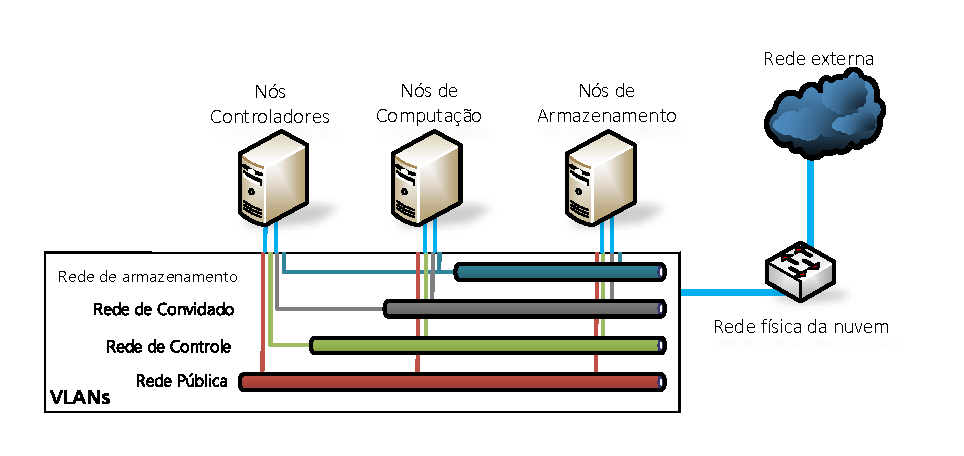
\includegraphics[width=1\textwidth]{img/topologia_generica.pdf}
	\label{fig:topologiaNuvemGenerica}\\
	Fonte: O próprio autor.
\end{figure}

Cada um destes hosts estão interligados através de duas interfaces de rede física (em azul claro na figura), e portanto, o uso de \ac{vlan} é necessário para isolar as quatro redes, que compartilham o meio físico. % @TODO -> verificar se devo alterar (em azul claro na figura)
%
Na parte de software, a utilização dos recursos destes hosts é feito pelo OpenStack, que disponibiliza suas funcionalidades para o consumidor através dos vários serviços instalados.
%
Neste sentido, este trabalho foca na caracterização voltada para os serviços mais populares, segundo \citeonline{openstack:about}: Glance, Keystone, Cinder, Swift, Nova e Neutron.
%
Em relação ao tráfego gerado por estes serviços, este trabalho planeja caracterizar aspectos do tráfego de controle que relacionem-se com o seu comportamento e desempenho.

Dentre os cenários de análise, planeja-se observar, por exemplo, o impacto de eventos periódicos no tráfego de controle, como no caso do serviço Nova solicitar a lista de \acp{vm} ativas.
%
Análises de comportamento geral também serão realizadas, que inclui, por exemplo, uma análise longitudinal, classificando o uso de banda dos serviços executando na nuvem.
%
Outro caso previsto é a caracterização do tráfego em tarefas específicas na nuvem, como o ciclo de vida de uma instância de \ac{vm} (\textit{e.g.,} criação de uma instância, ilustrado na Figura \ref{fig:openstack_criacao_instancia}).
%
Estas são expectativas gerais do que espera-se analisar, mas conforme a análise dos dados obtidos for feita é possível que outras conclusões surjam.
%
Um dos passos iniciais neste TCC, a análise de trabalhos com escopo semelhante tem sua importância neste processo, na qual analisa-se estudos que utilizam métricas e métodos aplicáveis neste trabalho.

\section{Trabalhos Relacionados}
\label{cap2:relacionados}

Para nortear o desenvolvimento da abordagem de medição e análise de tráfego proposta neste trabalho, esta seção apresenta outros trabalhos que têm o escopo ou objetivo similar, na qual monitoram e/ou caracterizam o tráfego em nuvens computacionais.
%
Ao apresentar os trabalhos busca-se explicar brevemente o contexto e objetivos deles, e então aprofundar em características, métricas e ferramentas que auxiliem na definição da proposta para caracterização de tráfego.
%
Após expor cada trabalho individualmente, a seção \ref{cap2:comparacao_trabalhos} apresenta uma discussão e comparação entre as abordagens contidas nos trabalhos.

\subsection{Venzano e Michiardi (2013)}

O trabalho de \citeonline{venzano:2013:trafficprivatecloud} investiga o impacto da virtualização no desempenho de comunicação em rede de aplicações com grande volume de dados em uma nuvem privada OpenStack.
%
Para monitorar o tráfego gerado, desenvolveram a ferramenta de monitoramento OSMeF (OpenStack \textit{Measurement Framework}), que executa sobre a ferramenta \texttt{nuttcp} para coletar métricas como vazão TCP e uso de CPU.
%
Em relação aos testes, o Hadoop é a aplicação distribuída escolhida em função da intensa troca de mensagens.
%
A aplicação foi alocada em um host para controlá-la e em outras dois hosts para realizar o processamento, além destes, outro host ficou responsável por hospedar serviços do OpenStack.

Neste trabalho foram realizadas duas caracterizações: \textbf{(I)} desempenho da interface de \textit{Loopback} em \acp{vm}; e \textbf{(II)} comparação da comunicação entre \acp{vm} no mesmo nó e em nós diferentes.
%
A caracterização \textbf{(I)} realizou-se diretamente na \ac{vm}, e verificou-se o desempenho da interface com diferentes quantidades de processadores.
%
A caracterização \textbf{(II)} foi realizada no Domínio de Convidado, que contém a rede física na qual as aplicações em execução nas \acp{vm} têm acesso e comunicam-se.
%
Não é explícito onde que a ferramenta de monitoramento (OSMeF) executa nos testes, mas em \textbf{(II)}, pelas métricas coletadas (\textit{i.e.,} uso de CPU), e a abordagem passiva de medição, é necessário monitorar cada host que executa a aplicação distribuída.
%
Outra característica é que a ferramenta necessita executar à nível de \textit{hypervisor} para acessar diretamente a interface física de rede do nó.
%
O processo de medição de tráfego neste trabalho utiliza diretamente a maioria das métricas coletadas (\textit{i.e.,} uso de CPU, vazão TCP), e apenas no caso da métrica ``Índice de justiça de Jain'' \cite{jain:1984:fairnessIndex} houve cálculo pós coleta.
%
Dentre os resultados obtidos destacam-se: há menor desempenho em interfaces \textit{Loopback} num ambiente virtualizado; e a comunicação entre \acp{vm} em um mesmo host possui melhor qualidade do que quando são distribuídas entre múltiplos hosts.


\subsection{Sciammarella et al. (2016)}

O trabalho de \citeonline{Sciammarella:2016:controltraffic} caracteriza o tráfego do Domínio de Controle de uma nuvem OpenStack geodistribuída, buscando entender o impacto da comunicação entre os nós controladores da nuvem e os nós de processamento em diferentes cenários. 
%
O ambiente de testes simula uma nuvem OpenStack distribuída entre universidades e centros de pesquisa. 
%
Na realização de um dos testes e sua respectiva medição de tráfego foi utilizada a ferramenta Rally\footnote{\url{https://wiki.openstack.org/wiki/Rally}}, que possibilita realizar \textit{benchmark} do OpenStack em diferentes cenários.
%
Como resultado, este trabalho buscou analisar como a execução de instâncias e outros serviços impacta na rede de controle.

Foram realizados três testes neste trabalho: \textbf{(I)} impacto do número de servidores de armazenamento e processamento, \textbf{(II)} impacto do número de \acp{vm} por servidor de armazenamento e processamento, e \textbf{(III)} impacto da criação e destruição de múltiplas \acp{vm}.
%
Nos três testes a caracterização de tráfego utilizou medição de tráfego passiva para realizar a coleta de tráfego, que focaram em analisar o uso de banda.
%
O teste \textbf{(I)} analisou o \textit{middleware} de comunicação RabbitMQ, e o MySQL, que são utilizados em múltiplos serviços, e separou o uso de banda de cada um em função do tempo decorrido.
%
Similarmente, no teste \textbf{(II)}, analisou-se o uso de banda no Domínio de Controle após a criação de quantidades variadas de \ac{vm} dentro de um ambiente controlado, sem categorizar as aplicações.
%
Não foi especificada a ferramenta de monitoramento empregada nos testes \textbf{(I)} e \textbf{(II)}. 
%
O teste \textbf{(III)} utilizou a ferramenta Rally, que permite realizar os testes e coletar os dados de maneira automatizada, executando situações que simulam diferentes cargas na nuvem.
%
Para realizar os testes, o Rally comunica-se com a nuvem OpenStack através da \ac{api}, realizando ações na nuvem conforme definido no \textit{script} sendo executado.
%
Em relação à coleta de dados, não é definida de maneira clara na documentação da ferramenta como ela ocorre.
%
Para o teste \textbf{(III)}, o \textit{script} definido foi criação e destruição de múltiplas instâncias, que então coletou o tráfego gerado pela tarefa, buscando entender o uso de banda resultante em função das requisições.
%
Não há como confirmar se houve uso exclusivo da ferramenta Rally na etapa de medição de tráfego, que é algo plausível levando em conta a similaridade das métricas analisadas.


\subsection{Wang e Ng (2010)}

O trabalho de \citeonline{Wang:2010:ec2networkperformance} caracteriza o tráfego de rede entre \acp{vm} com um e dois processadores virtuais hospedados na \textit{Amazon Elastic Cloud Computing} (EC2).
%
O objetivo é identificar o impacto da virtualização no desempenho da rede, com alguns objetivos específicos, como verificar se há compartilhamento de processador entre duas \acp{vm} de apenas um processador virtual cada, e o impacto resultante na comunicação.
%
Realizaram-se dois testes que avaliaram o uso de processador e características de rede como: vazão TCP e UDP, atraso na transmissão, e perda de pacote.
%
Nos dois testes foram empregadas as mesma ferramentas: \texttt{ping} para calcular o atraso na comunicação, ferramentas autorais para vazão TCP e UDP, e a ferramenta Badabing \cite{sommers:2005:badabing} para estimar a perda de pacote correspondente.
% 
Como resultado, concluiu-se que há, de fato, compartilhamento de processador nas \acp{vm} mais simples ofertadas pelo serviço Amazon EC2, e que este compartilhamento de processador resulta em instabilidade na transmissão de dados pela rede, variando rapidamente entre 1GB/s e zero GB/s.

Em relação aos testes, ambos analisaram as mesmas métricas, mas sob perspectivas diferentes, em dois teste: teste espacial, e teste temporal.
%
O teste espacial realizou as medições em 750 \acp{vm} de 1 processador e 150 \acp{vm} de 2 processadores, no total, com duração aproximada de 10 segundos cada.
%
O teste temporal efetuou as medições em 6 \acp{vm} de 1 processador e 3 \acp{vm} de 2 processadores ao longo de 150 horas cada.
%
Em relação às ferramentas empregadas, todas utilizam medição ativa de tráfego, ou seja, fizeram a medição com base nos pacotes criados pela próprias ferramentas.
%
As ferramentas autorais para medição de TCP e UDP funcionam de maneira similar, executando duas instâncias das ferramentas em \acp{vm} diferentes, e calculando as métricas resultantes com base na comunicação entre elas.
%
A ferramenta Badabing é executada em duas \acp{vm}, e a cada 5ms realiza o envio de pacotes e cálculo da métrica de perda de pacote.


\subsection{Sharma et al. (2014)}

O trabalho de \citeonline{sharma:2015:hansel} desenvolveu o Hansel, um sistema de detecção de falhas para nuvens baseadas em OpenStack.
%
Este sistema monitora o Domínio de Controle, buscando identificar padrões na comunicação entre serviços que caracterizem a ocorrência de falhas.
%
Durante a execução, o Hansel analisa cada mensagem enviada pelos serviços através de \ac{rpc} e REST, buscando algum identificador único pertencente àquela cadeia de eventos.
%
A partir do identificador cria-se um grafo direcionado, que corresponde à uma cadeia de eventos gerado por uma requisição REST.
%
Mensagens \ac{rpc} são agregadas definidas como auto transições no nó mais recente do grafo, que corresponde à mensagem REST mais recente.
%
Esta agregação de mensagens \ac{rpc} é necessário por sua quantidade ser maior do que de mensagens REST, e também ao fato de que mensagens REST necessitarem de menos processamento para identificar o par no qual pertencem.
%
Falhas são diagnosticados ao identificar uma mensagem REST na cadeia de eventos que contém algum código de erro.
%
Ao identificá-la, retorna-se então ao início do grafo para determinar a sequência de eventos que levaram à falha.

A arquitetura de instalação divide o sistema de monitoramento Hansel em duas partes: agentes monitores e serviço de análise central.
%
Para ter acesso a todas as mensagens emitidas, os agentes monitores executam em todos nós de controle e de computação pertencentes à nuvem em questão.
%
Estes agentes monitores foram implementados sobre a ferramenta Bro \cite{paxson:1999:bro}, que através da \ac{api}, chamada Broccoli, possibilitou o \textit{parse} das mensagens do OpenStack em Python.
%
Estes agentes monitores realizam a medição passiva de tráfego, enviando para o serviço de análise central o contexto extraído das mensagens.
%
O contexto é composto pelo identificador da mensagem, que pode ser extraído do UUID ou do identificador atribuído pelo OpenStack, e de outros metadados como: origem e destino da mensagem, protocolo (\textit{e.g.,} REST ou \ac{rpc}), e o conteúdo da mensagem. 
%
A geração dos identificadores é atribuída aos agentes monitores para diminuir a carga no serviço de análise central, que efetua o resto do processamento (\textit{e.g.,} geração dos grafos, identificação de falha).
%
Segundo os autores, o Hansel não depende de um formato específico de mensagem nos protocolos REST e \ac{rpc}, e portanto pode ser aplicado em outras versões do OpenStack Juno, que foi a versão testada.
%
Durante os testes realizados, o sistema de monitoramento funcionou adequadamente com a transmissão de até 1.600 mensagens REST e \ac{rpc} por segundo no tráfego do Domínio de Controle.

\subsection{Análise e comparação dos trabalhos relacionados}
\label{cap2:comparacao_trabalhos}

Esta seção expõe uma análise sobre os trabalhos relacionados apresentados.
%
Em específico, são apontadas características relevantes a cada trabalho, e após é feita uma comparação entre estas características.
%

Para evidenciar as características comparadas, a Tabela \ref{tab:trab_relacionados_ambiente} e Tabela \ref{tab:trab_relacionados_metrica} apresentam os mesmos trabalhos, mas com diferentes características avaliadas.
%
Na Tabela \ref{tab:trab_relacionados_ambiente} são apresentadas três características, na qual a primeira delas define o objetivo final daquele trabalho.
%
A segunda característica apresentada na tabela define qual domínio, conforme apresentado na Seção \ref{cap2:openstack_network_architecture}, este trabalho analisa.
%
A terceira e última característica desta tabela define o ambiente de computação em nuvem utilizado no trabalho.
%
A Tabela \ref{tab:trab_relacionados_metrica} apresenta outras três características, cuja primeira característica define qual o tipo de medição que as ferramentas utilizadas empregam.
%
A segunda característica define as métricas utilizadas para caracterizar o tráfego ou avaliar o sistema de monitoramento implementado.
%
A terceira e última característica apresentada nesta tabela são as ferramentas produzidas ou empregadas no trabalho para alcançar o seu objetivo.

\begin{table}[!htb]
\centering
\footnotesize
\caption{Análise comparativa dos trabslhos relacionados: objetivo do trabalho, rede alvo, e ambiente}
\begin{tabularx}{\textwidth}{XlXl}
\hline
\multicolumn{1}{c|}{\textbf{Trabalho}} & \multicolumn{1}{c|}{\textbf{Objetivo do trabalho}} & \multicolumn{1}{c|}{\textbf{Domínio alvo}} & \multicolumn{1}{c}{\textbf{Ambiente}} \\ \hline
Venzano e Michiardi (2013) & Caracterização de tráfego & Domínio de Convidado & OpenStack \\
\rowcolor[HTML]{EFEFEF} 
Sciammarella et al. (2016) & Caracterização de tráfego & Domínio de Controle & OpenStack \\
Wang e Ng (2010) & Caracterização de tráfego & Domínio de Convidado & Amazon EC2 \\
\rowcolor[HTML]{EFEFEF} 
Sharma et al. (2014) & Monitoração de tráfego & Domínio de Controle & OpenStack \\ \hline\end{tabularx}
\label{tab:trab_relacionados_ambiente}\\
Fonte: O próprio autor.
\end{table}

Na Tabela~\ref{tab:trab_relacionados_ambiente}, dos quatro trabalhos analisados, três realizam a caracterização de tráfego de nuvens computacionais como objetivo final, e utilizam ferramentas para medição de tráfego como meio para atingir este objetivo.
%
Um trabalho desenvolveu um sistema para monitoramento de tráfego, na qual realiza a busca por falhas como objetivo final.
%
Esta diferença nos objetivos reflete na aplicação de métricas, que no caso dos trabalhos que caracterizam o tráfego, as métricas são empregadas no processo de caracterização, enquanto que no sistema de monitoramento, as métricas avaliam o desempenho do sistema.
%
Este TCC realizará os dois objetivos, na qual monitorará algumas características da rede em tempo real, e então, fará uma caracterização do tráfego com uma abordagem longitudinal.

Continuando a interpretação da Tabela~\ref{tab:trab_relacionados_ambiente}, os domínios definidos na coluna ``Domínio alvo'' remetem à Seção~\ref{cap2:openstack_network_architecture}, que por conta da definição genérica, também podem ser aplicados em outros sistemas de gerenciamento de nuvem computacional.
%
Contudo, não há como ter permissão de acesso ao Domínio de Controle em nuvens públicas sem explorar algum tipo de falha no sistema, logo, a análise deste domínio está restrita a nuvens privadas, como as construídas com o OpenStack.
%
A análise do Domínio de Convidado é possível em qualquer nuvem \ac{iaas} que o consumidor tenha acesso a \acp{vm} e possa executar ferramentas para medir o tráfego na sua rede virtualizada conforme as métricas escolhidas.
%
Neste sentido, no caso de trabalhos no ambiente Amazon EC2, não é possível monitorar e posteriormente caracterizar o tráfego do Domínio de Controle.
\pagebreak

\begin{table}[!htb]
\centering
\scriptsize
\caption{Análise comparativa dos trabalhos relacionados: tipo de medição, métricas, e ferramentas}
\begin{tabularx}{\textwidth}{XXXX}
\hline
\multicolumn{1}{c|}{\textbf{Trabalho}} & \multicolumn{1}{c|}{\textbf{Tipo de medição}} & \multicolumn{1}{c|}{\textbf{Métricas}}           & \multicolumn{1}{c}{\textbf{Ferramentas}} \\ \hline
Venzano e Michiardi (2013)             & \multicolumn{1}{l}{Passiva}                              & Uso de CPU; Vazão TCP; Índice de Justiça de Jain & Autoral (implementado sobre Nuttcp)      \\
\rowcolor[HTML]{EFEFEF} 
Sciammarella et al. (2016)             & \multicolumn{1}{l}{Passiva}                                                  & Uso de banda por serviço; Uso de banda da rede   & Rally; Desconhecida                      \\
Wang e Ng (2010)                       & \multicolumn{1}{l}{Ativa}                                                    & Vazão TCP, Vazão UDP; Atraso; Perda de pacote    & Badabing; Ping; Autoral                  \\
\rowcolor[HTML]{EFEFEF} 
Sharma et al. (2014)                   & \multicolumn{1}{l}{Passiva}                                                  & Uso de CPU; Uso de memória                       & Hansel (implementado sobre Bro)          \\ \hline
\end{tabularx}
\label{tab:trab_relacionados_metrica}\\
Fonte: O próprio autor.
\end{table}

Na Tabela~\ref{tab:trab_relacionados_metrica}, em ambos os tipos de trabalho foram empregadas ferramentas para realizar a medição do tráfego, pois independente do objetivo, seja caracterização ou apenas monitoramento, é necessário coletar o tráfego.
%
Para realizar o processo de medição de maneira mais rápida e eficiente todos os trabalhos utilizaram ferramentas já conhecidas ou realizaram suas próprias implementações sobre ferramentas já existentes.
%
Em relação às ferramentas prontas, o Badabing e o Rally foram aplicados diretamente na etapa de medição de tráfego, na qual o Badabing foca apenas na métrica de perda de pacote, e o Rally disponibiliza várias métricas, que são escolhidas de acordo com o escopo do trabalho.

Implementações em \cite{sharma:2015:hansel,venzano:2013:trafficprivatecloud} foram realizadas sobre duas ferramentas, respectivamente: Bro e \texttt{Nuttcp}.
%
O \texttt{Nuttcp} foi utilizado para dispensar a preocupação com a lógica em mais baixo nível, relacionado com a coleta de métricas do uso de CPU e interface de rede física.
%
A ferramenta Bro oferece uma plataforma, e que ao usar sua \ac{api}, é possível enviar e receber mensagens através do seu protocolo, além de poder acessar várias outras funcionalidades relacionadas com o monitoramento do tráfego de rede.
%
O trabalho \cite{Sciammarella:2016:controltraffic} não descreveu a ferramenta empregada na realização de dois cenários durante a caracterização de tráfego, na qual envolviam analisar o uso de banda de certas aplicações e o uso de banda geral da rede, respectivamente.

As métricas escolhidas nos trabalhos, apesar de semelhantes, são aplicadas em contextos diferentes, e neste sentido impossibilita uma comparação direta. 
%
O trabalho de \citeonline{venzano:2013:trafficprivatecloud} focou no contexto de aplicações distribuídas, e avaliou como o local na qual as \acp{vm} estão alocadas influenciam no desempenho resultante.
%
Em relação à \citeonline{Wang:2010:ec2networkperformance}, a análise é mais elementar, cujo objetivo é descobrir qual a qualidade dos recursos de rede disponibilizados conforme o serviço contratado da EC2.
%
As métricas adotadas por \citeonline{Sciammarella:2016:controltraffic} avaliam qual o uso de recurso de rede  de uma nuvem conforme a escala da nuvem.
%
Com os valores base definidos, é possível estimar até onde uma nuvem pode crescer e oferecer um serviço de qualidade.
%
As métricas adotadas em \citeonline{sharma:2015:hansel} avaliam o uso de recursos pelo sistema de monitoramento, cujo um valor alto, por exemplo, aponta que monitorar a rede pode não ser viável, e valores baixos indicam sua viabilidade.

Este TCC pretende caracterizar o comportamento do Domínio de Controle, e portanto, parte da análise será voltada para métricas de desempenho.
%
A outra parte da análise pretende avaliar comportamentos que ocorrem no Domínio de Controle, mas que talvez não sejam documentados pelo OpenStack, e portanto, não podem ser expressos em métricas.

\section{Considerações do capítulo}
\label{cap2:consideracoes}

Este capítulo conceituou computação em nuvem, o sistema de gerenciamento de nuvem OpenStack e abordagens existentes na caracterização de tráfego.
%
Após apresentar sobre computação em nuvem detalha-se sobre como é realizada a virtualização e qual a sua influência no funcionamento de recursos computacionais.
%
Então, após uma introdução sobre o OpenStack, são descritos alguns serviços que fornecem funcionalidades para a nuvem e a arquitetura de rede recomendada em uma instalação.
%
A última parte da conceitualização expõe uma maneira de abordar a caracterização de tráfego, dividindo-a em duas etapas: medição de tráfego e análise de tráfego.

As seções após a conceitualização descrevem sobre o escopo do problema abordado neste TCC, relacionando-os com os conceitos apresentados.
%
A primeira seção relacionada ao escopo do trabalho define o problema a ser tratado nesse TCC, na qual exemplifica-o aplicando alguns dos conceitos apresentados.
%
Então, para fundamentar melhor o escopo deste TCC, são analisados características e ferramentas contidas em trabalhos relacionados, cuja análise auxilia na criação de uma proposta.
